
\let\negmedspace\undefined
\let\negthickspace\undefined
\documentclass[journal]{IEEEtran}
\usepackage[a5paper, margin=10mm, onecolumn]{geometry}
%\usepackage{lmodern} % Ensure lmodern is loaded for pdflatex
\usepackage{tfrupee} % Include tfrupee package
\setlength{\headheight}{1cm} % Set the height of the header box
\setlength{\headsep}{0mm}     % Set the distance between the header box and the top of the text
\usepackage{gvv-book}
\usepackage{gvv}
\usepackage{cite}
\usepackage{amsmath,amssymb,amsfonts,amsthm}
\usepackage{algorithmic}
\usepackage{graphicx}
\usepackage{textcomp}
\usepackage{xcolor}
\usepackage{txfonts}
\usepackage{listings}
\usepackage{enumitem}
\usepackage{mathtools}
\usepackage{gensymb}
\usepackage{comment}
\usepackage[breaklinks=true]{hyperref}
\usepackage{tkz-euclide} 
\usepackage{listings}
% \usepackage{gvv}                                        
\def\inputGnumericTable{}                                 
\usepackage[latin1]{inputenc}                                
\usepackage{color}                                            
\usepackage{array}                                            
\usepackage{longtable}                                       
\usepackage{calc}                                             
\usepackage{multirow}                                         
\usepackage{hhline}                                           
\usepackage{ifthen}                                           
\usepackage{lscape}
\renewcommand{\thefigure}{\theenumi}
\renewcommand{\thetable}{\theenumi}
\setlength{\intextsep}{10pt} % Space between text and floats
\numberwithin{equation}{enumi}
\numberwithin{figure}{enumi}
\renewcommand{\thetable}{\theenumi}
\begin{document}
\bibliographystyle{IEEEtran}
\title{Question 1-1.8-5q}
\author{EE24BTECH11015 - Dhawal}
% \maketitle
% \newpage
% \bigskip
{\let\newpage\relax\maketitle}
\begin{enumerate}
	\item If $\vec{A}$ and $\vec{B}$ be the points $\brak{3,4,5}$ and $\brak{-1,3,-7}$ respectively, find the equation of the set of points $\vec{P}$ such that ${PA}^2+{PB}^2=K^2$ where $K$ is a constant.
\end{enumerate}
\begin{table}[h!]    
  \centering
  
\begin{tabular}[12pt]{ |c| c| c|}
    \hline
    \textbf{Variable} & \textbf{Description} & \textbf{Values} \\ 
    \hline
    AB & Length & 6 cm \\
    \hline
    BC & Length & 8 cm \\
    \hline
    $\angle ABC$ & Angle & \ang{60}\\
    \hline 
    $\vec{A}$ & Point & $(6,0)$ \\
    \hline
    $\vec{B}$ & Origin & $(0,0)$ \\
    \hline
    $\vec{C}$ & To find & ? \\
    \hline
    \end{tabular}


  \caption{Variables Used}
  \label{tab 1.4.9.2}
\end{table}
Solution:\\
Solving the equation,
\begin{align}
        {PA}^2+{PB}^2=K^2
        \end{align}
        \begin{align}
        \mydet{\mydet{\vec{P}-\vec{A}}}^2+\mydet{\mydet{\vec{P}-\vec{B}}}^2=K^2
        \end{align}
        \begin{align}
        \brak{\vec{P}-\vec{A}}^{T} \brak{\vec{P}-\vec{A}}+\brak{\vec{P}-\vec{B}}^{T}\brak{\vec{P}-\vec{B}}=K^2
        \end{align}
        \begin{align}
        \mydet{\mydet{\vec{P}}}^2 -\vec{P}^{T}\vec{A}-\vec{A}^{T}\vec{P}+\mydet{\mydet{\vec{A}}}^2 +\mydet{\mydet{\vec{P}}}^2 -\vec{P}^{T}\vec{B}-\vec{B}^{T}\vec{P}+\mydet{\mydet{\vec{B}}}^2 =K^2
\end{align}
For vectors,
\begin{align}
	\vec{P}^{T}\vec{A}=\vec{A}^{T}\vec{P} \text{ and } \vec{P}^{T}\vec{B}=\vec{B}^{T}\vec{P}
\end{align}
Then,
\begin{align}
	2\mydet{\mydet{\vec{P}}}^2  -2\vec{A}^{T}\vec{P}+\mydet{\mydet{\vec{A}}}^2 -2\vec{B}^{T}\vec{P}+\mydet{\mydet{\vec{B}}}^2 =K^2
\end{align}
Equation without putting the values of $\vec{A}$ and $\vec{B}$,
\begin{align}
	2\mydet{\mydet{\vec{P}}}^2  -2\vec{A}^{T}\vec{P}+\mydet{\mydet{\vec{A}}}^2 -2\vec{B}^{T}\vec{P}+\mydet{\mydet{\vec{B}}}^2 -K^2=0
\end{align}
Finding $\mydet{\mydet{\vec{A}}}^2$,
\begin{align}
\mydet{\mydet{\vec{A}}}^2=\vec{A}^T\vec{A}=\myvec{3&4&5}\myvec{3\\4\\5}=50
\end{align}
Finding $\mydet{\mydet{\vec{B}}}^2$,
\begin{align}
\mydet{\mydet{\vec{B}}}^2=\vec{B}^T\vec{B}=\myvec{-1&3&-7}\myvec{-1\\3\\-7}=59
\end{align}
Putting the values in equation, 
\begin{align}
	2\mydet{\mydet{\vec{P}}}^2  -2\myvec{3&4&5}\vec{P}+50-2\myvec{-1&3&-7}\vec{P}+59-K^2=0
\end{align}
\begin{align}
	2\mydet{\mydet{\vec{P}}}^2  -\myvec{6&8&10}\vec{P}-\myvec{-2&6&-14}\vec{P}+109-K^2=0
\end{align}
Final equation:
\begin{align}
	2\mydet{\mydet{\vec{P}}}^2  -\myvec{4&14&-4}\vec{P}+109-K^2=0
\end{align}\begin{figure}[h!]
   \centering
   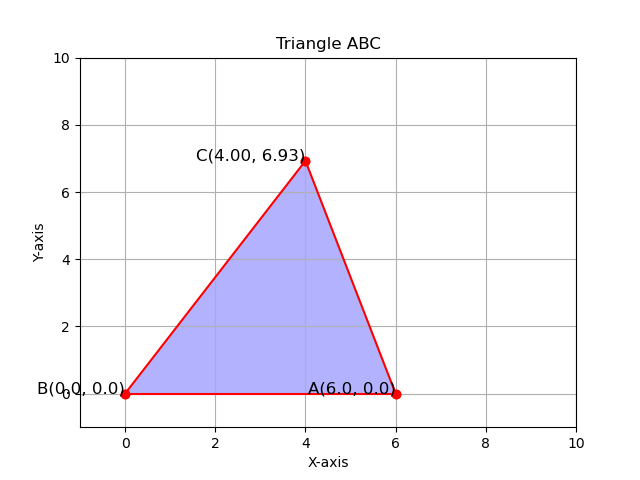
\includegraphics[width=0.9\linewidth]{Figure_1.png}
	\caption{Locus of P }
   \label{stemplot}
\end{figure}


\end{document}

